\documentclass{beamer}

\usepackage[utf8x]{inputenc}
\usepackage{default}
\usetheme{Warsaw}
\usepackage{beamerthemesplit}
\usecolortheme{rose}%Light definition headings
\usefonttheme[onlysmall]{structurebold}
\setbeamerfont{title}{shape=\itshape,family=\sffamily}
%\setbeamercolor{background canvas}{bg=red!20}
%\usefonttheme[onlylarge]{structuresmallcapsserif}%Large headings
%\setbeamercolor{title}{fg=red!80!black,bg=red!20!white}
%\mode<handout>{\beamertemplatesolidbackgroundcolor{black!5}}
\usepackage{pdfpages}
\usepackage{textcomp}
\usepackage{amsmath}
\usepackage{geometry}
%\usepackage{subfig}
\usepackage{float}
\usepackage{graphicx}
%\floatstyle{boxed}
%\restylefloat{figure}
\title{\texttt{EduAerospace}}
\subtitle{AE 663 : Software Development Techniques for Engineering and Scientists}
%\author{Thammisetty Devakumar - 08001021 \\ Mustafa Mutiur Rahaman - 08D01022 \\ Shiv Kailash V - 08001022}
\date{\empty}


\begin{document}

\begin{frame}[label = Titlepage]
	\titlepage
	\vspace*{-3cm}
	\begin{figure}
		\centering
		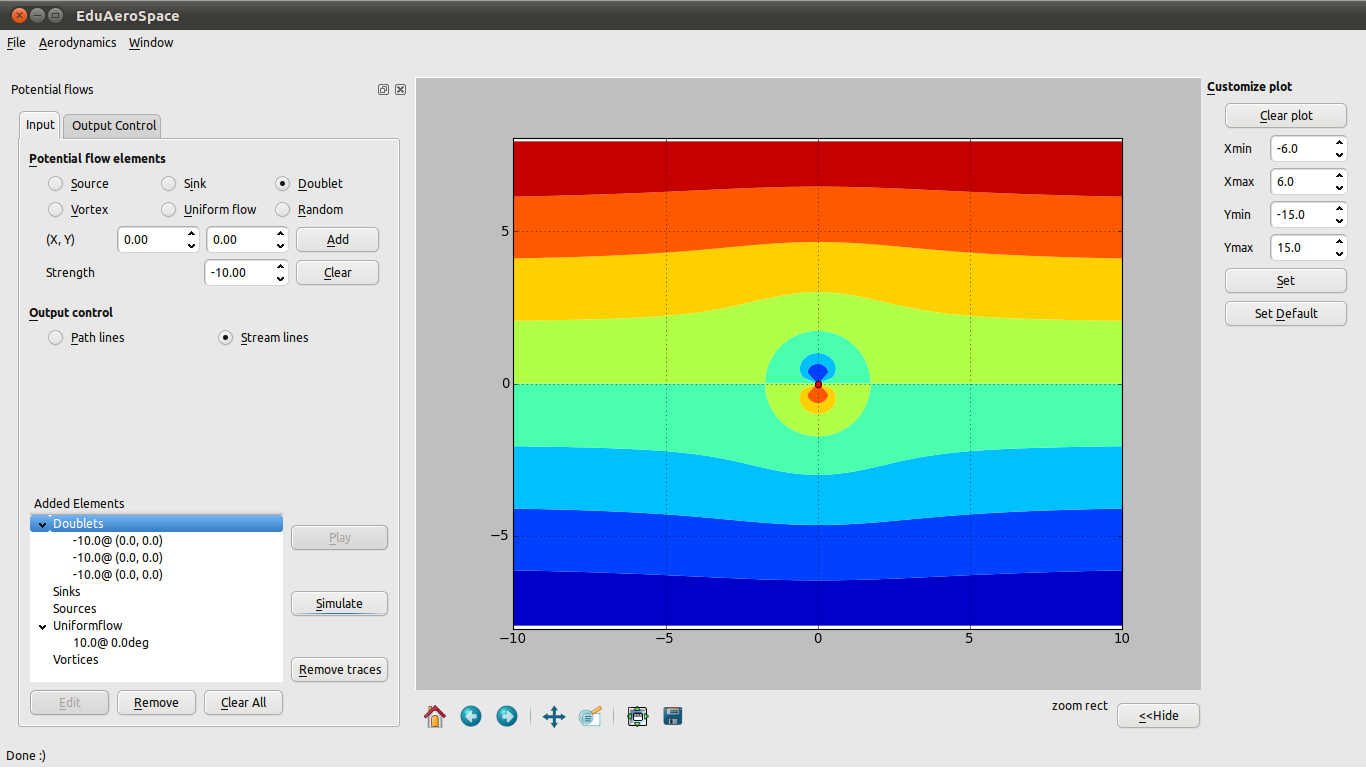
\includegraphics[width=0.8\textwidth]{Images/pic2.png}
	\end{figure}
\end{frame}

\section{Outline}
\begin{frame}[label = toc]
	\tableofcontents[pausesections]
\end{frame}

%\begin{frame}
%	\begin{figure}
%		\centering
%		\subfloat[Uniform Flow]{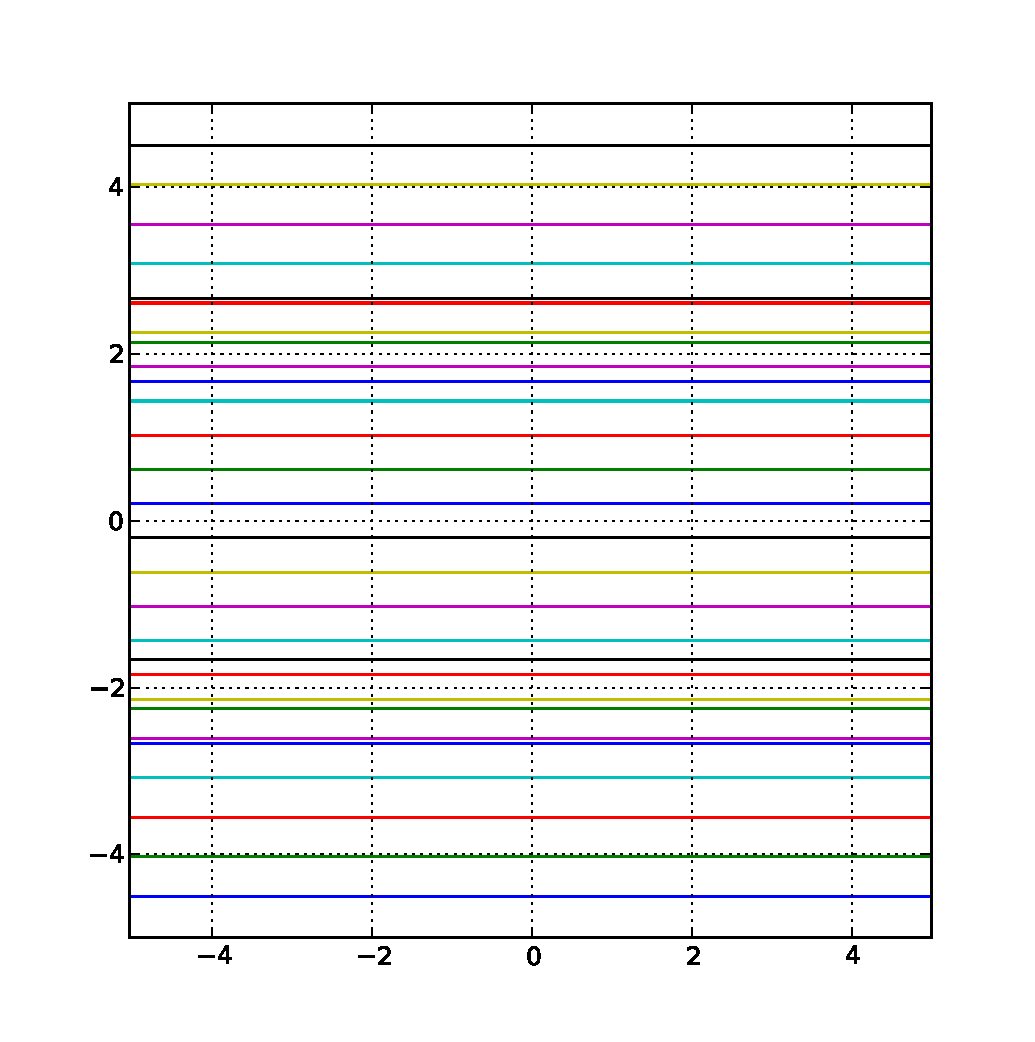
\includegraphics[width=0.45\textwidth]{Images/uniform.pdf}}
%		\subfloat[Source]{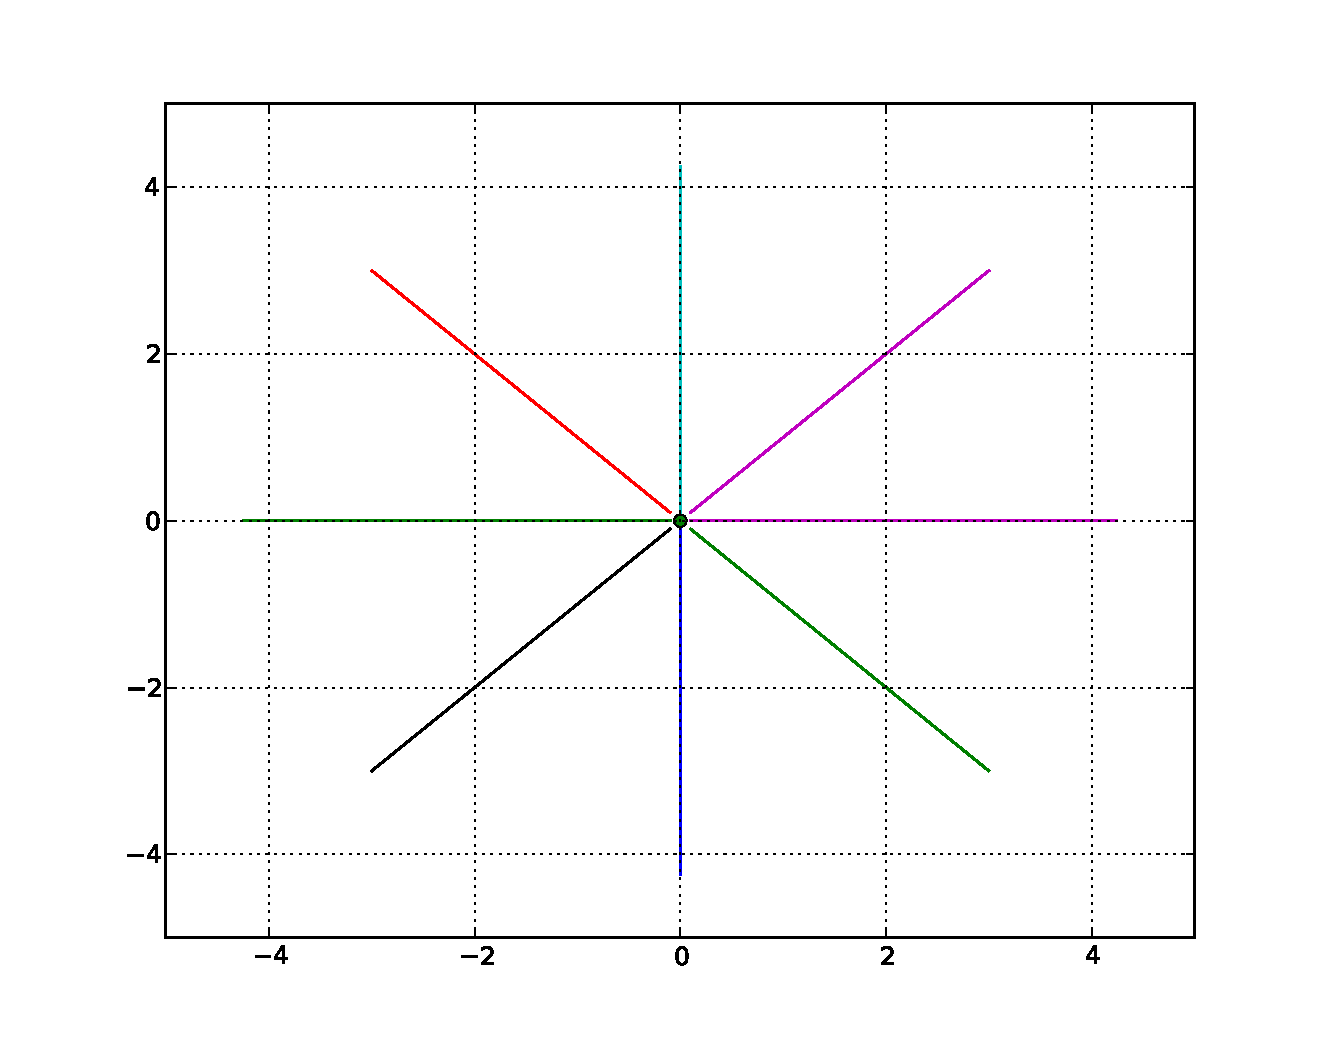
\includegraphics[width=0.45\textwidth]{Images/source.pdf}}
%		\subfloat[Doublet]{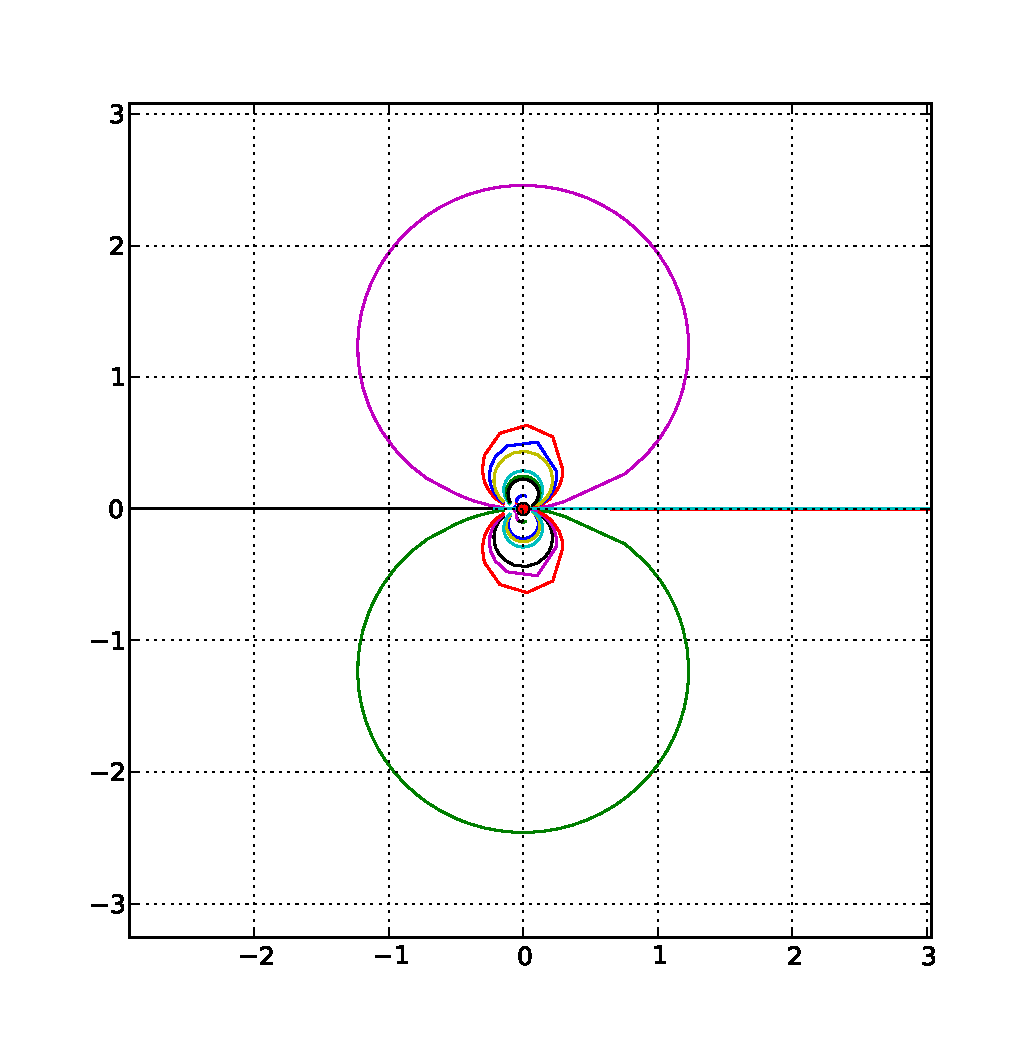
\includegraphics[width=0.45\textwidth]{Images/doublet.pdf}}
%		\subfloat[Vortex]{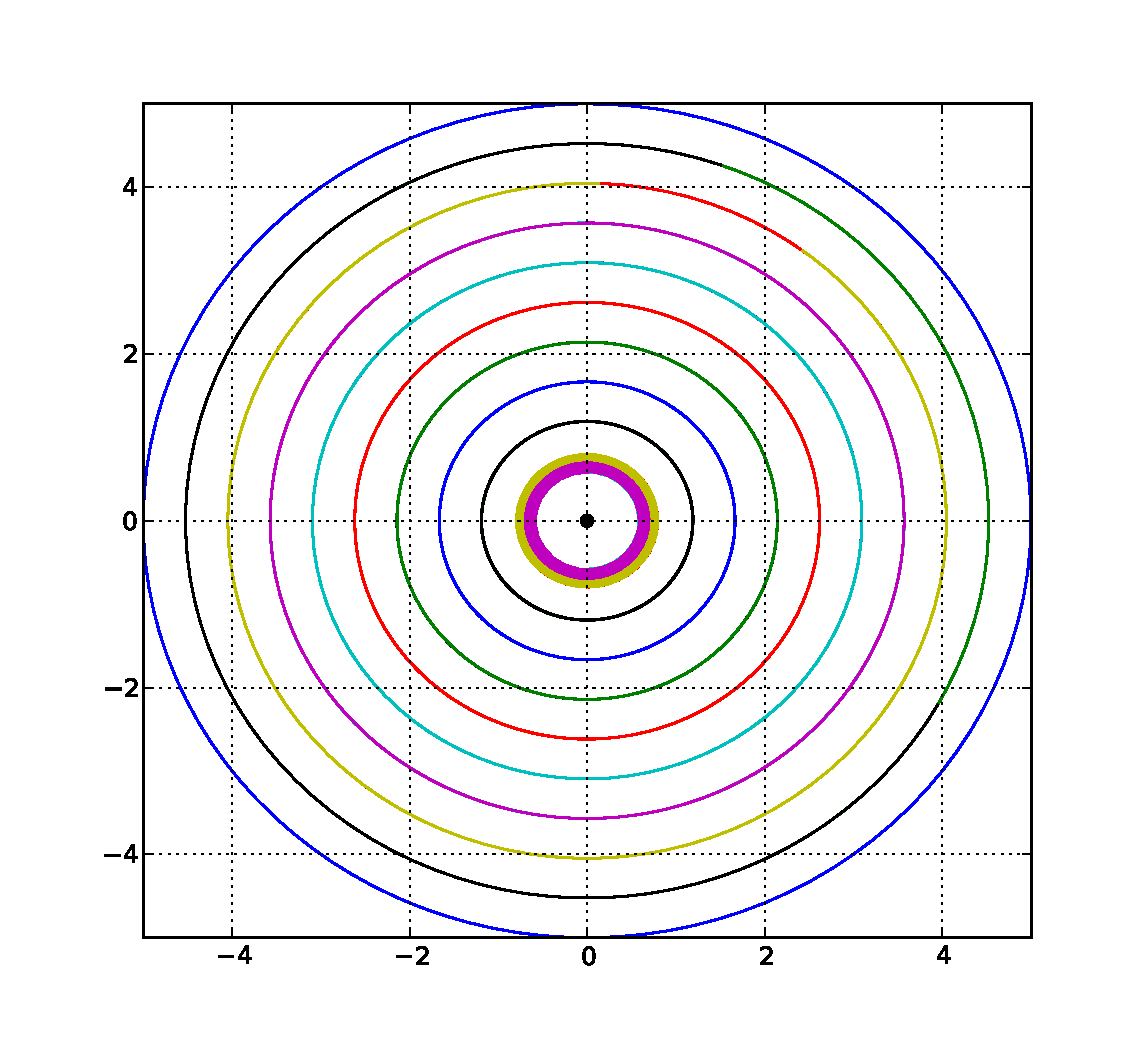
\includegraphics[width=0.45\textwidth]{Images/vortex.pdf}}
%		\caption{Potential flow elements}
%	\end{figure}
%\end{frame}

\section{Potential Flows}
\begin{frame}
	\frametitle{Basic Elements}
	\begin{figure}
		\centering
		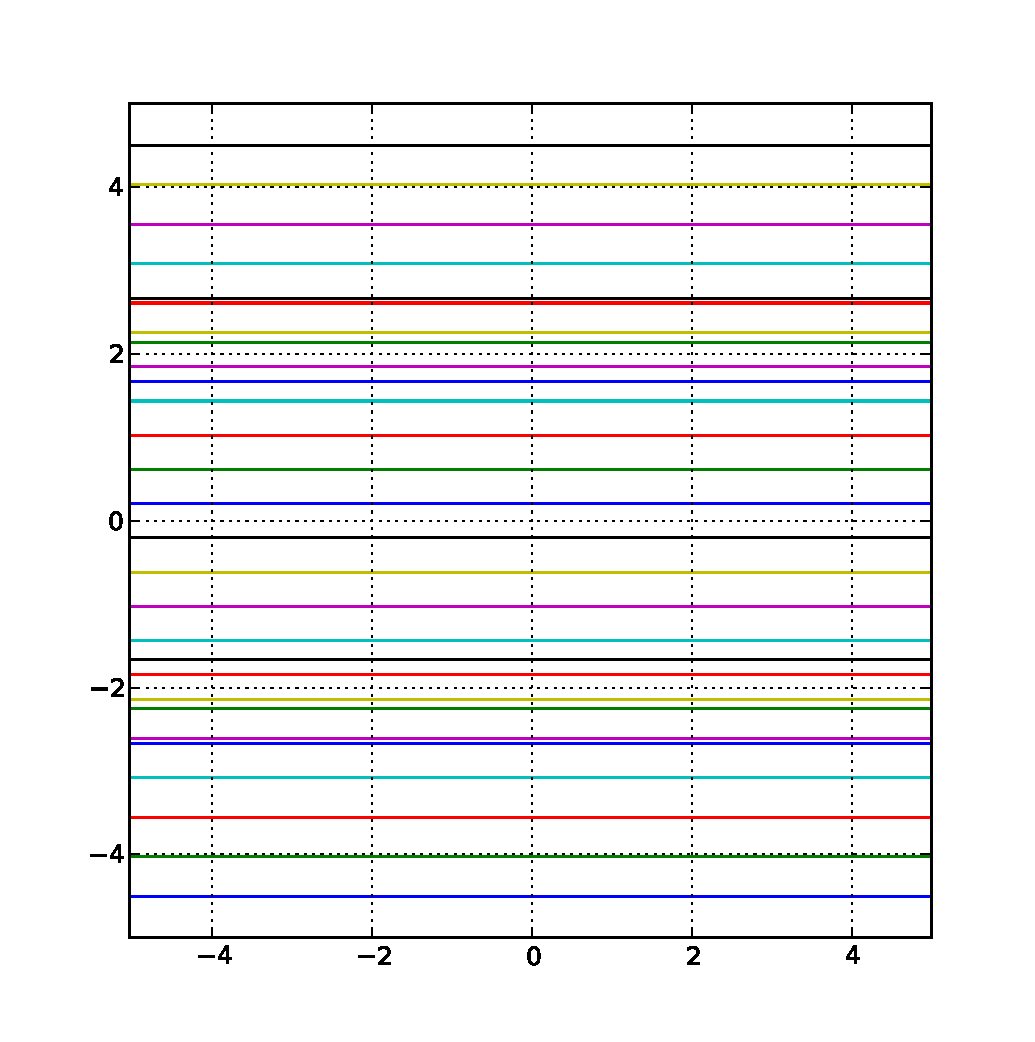
\includegraphics[width=0.3\textwidth]{Images/uniform.pdf}
		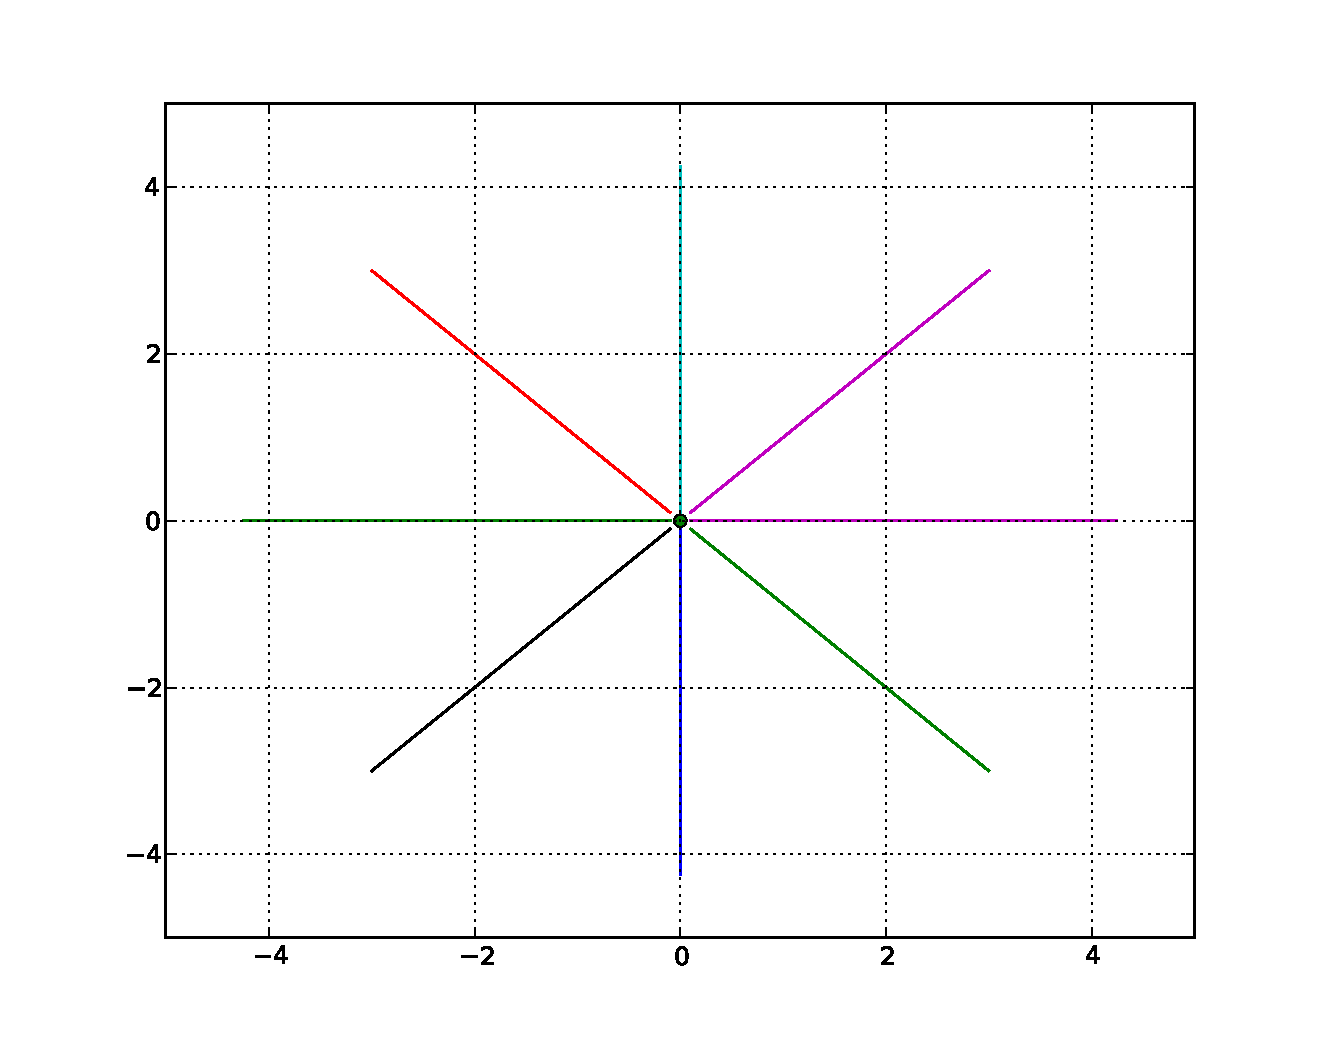
\includegraphics[width=0.3\textwidth]{Images/source.pdf}\\
		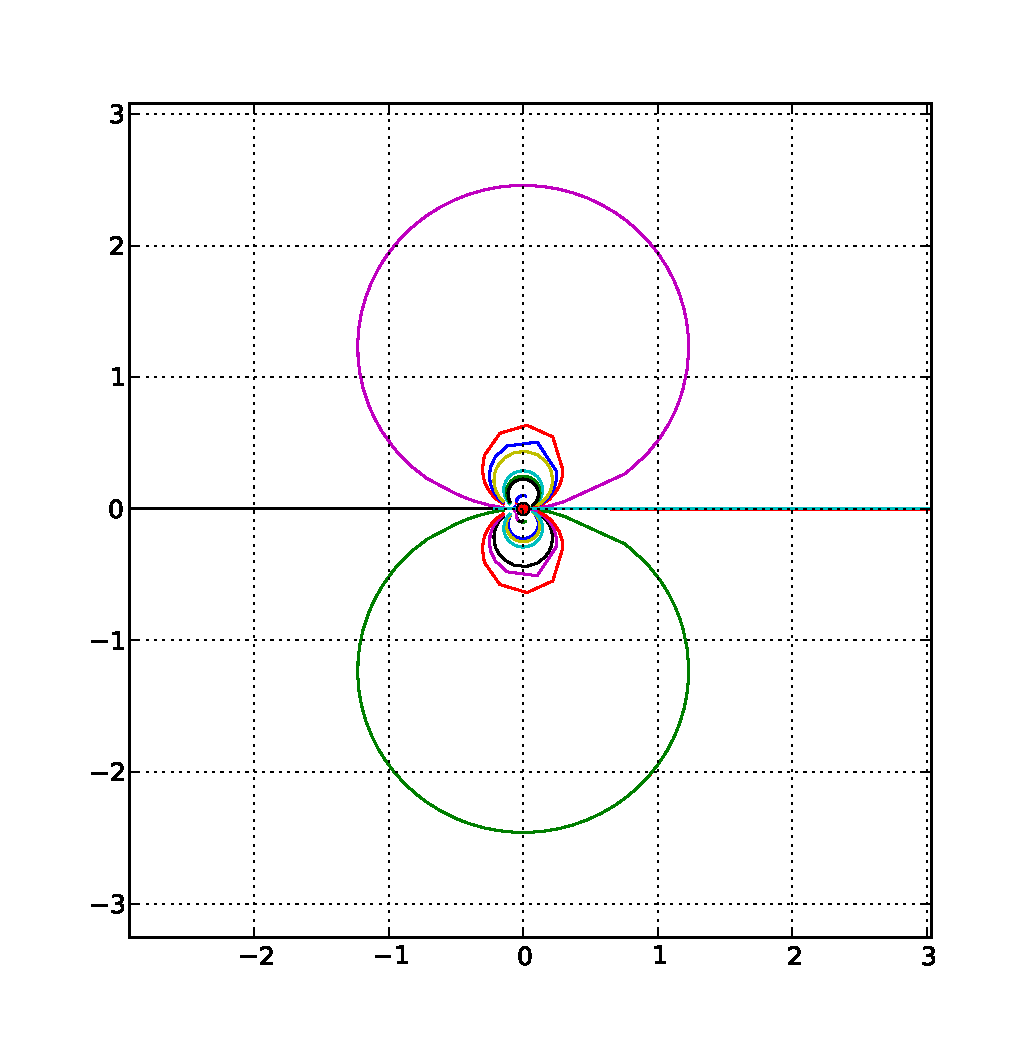
\includegraphics[width=0.4\textwidth]{Images/doublet.pdf}
		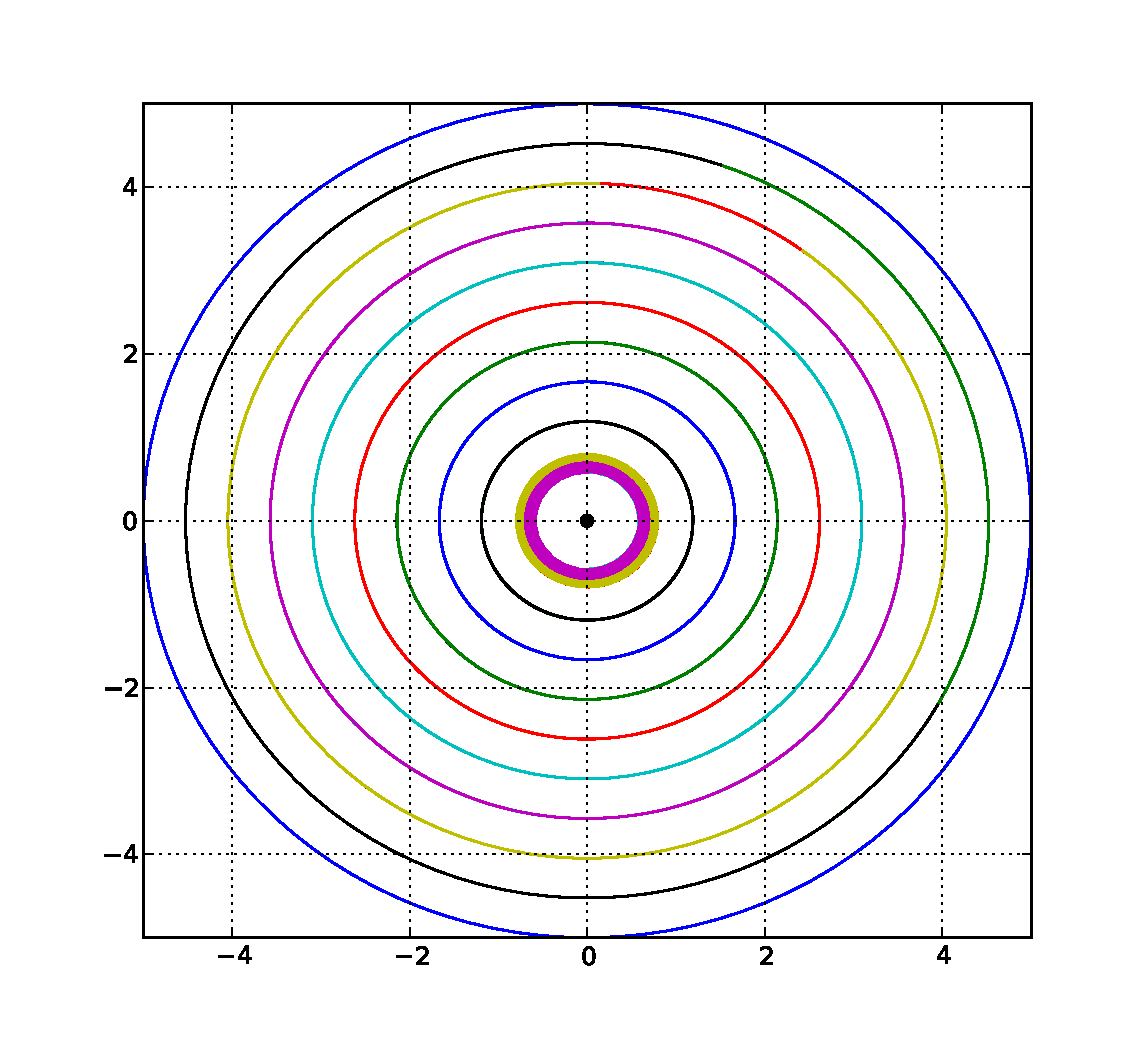
\includegraphics[width=0.4\textwidth]{Images/vortex.pdf}
%		\caption{Uniform Flow, Source}
	\end{figure}
\end{frame}

\begin{frame}
	\frametitle{Basic input features in GUI}
	\begin{itemize}
		\item Add desired potential elements
		\item Interactive plot : \alert{Add} $->$ will be shown in the figure, message in \alert{status bar}
		\item Auto resizing of plotwindow - Not using \alert{auto\_rescale(on)}
			\pause
		\item Can \alert{remove} the elements added!\ldots Also \alert{all} at once!!!
			\pause
		\item \alert{TODO : } Edit the elements added
	\end{itemize}
\end{frame}

\begin{frame}
	\frametitle{Basic output control features in GUI}
	\begin{itemize}
		\item Can plot stream lines - a bit \alert{slow}
	\begin{itemize}
			\item For axis whose length is \alert{10} units, 200$\times$300 values are being considered
			\pause
	\end{itemize}
		\item Tracking evolution of particles - \alert{real time}
			\pause
	\begin{itemize}
			\item Add particles at any desired locations
			\pause
			\item Add patches \begin{enumerate}
				\item At any \alert{X} or \alert{Y} location
				\item Square
				\item Circular
				\end{enumerate}
	\end{itemize}
			\pause
		\item \alert{TODO : } Release particles in rectangular, elliptical, parabolic, hyperbolic patches
	\end{itemize}
\end{frame}

\begin{frame}
	\frametitle{Additional features in GUI}
	\begin{itemize}
		\item Can \alert{play} or \alert{pause} the simulation 
			\pause
		\item Add/Remove elements. Can add new particle during simulation
		\item \alert{Delete} all the particles added for evolution.
			\pause
		\item \alert{Clear plot} without changing the current axis range
			\pause
		\item Can \alert{set} desired \alert{axis limits} for simulation!!!
	\end{itemize}
\end{frame}

\begin{frame}
	\frametitle{Features to be implemented}
	\begin{itemize}
		\item User option to select \alert{blob} to treat the simulation - Currently using \alert{Chorin} blob
			\pause
		\item Velocity, Velocity potential($\phi$) contours
			\pause
		\item Keyboard shortcuts in plot window: \alert{+} for zoom in..etc
			\pause
		\item Continuous potential elements implementation
	\end{itemize}
\end{frame}

\begin{frame}
	\begin{center}
		\Huge{Thank you}
	\end{center}
\end{frame}

\end{document}
